\documentclass[11pt]{article}
\usepackage{amsmath, amssymb, physics, mathtools, bm}
\usepackage{tikz, pgfplots}
\usetikzlibrary{calc, positioning}
\pgfplotsset{compat=1.18}
\usepackage[margin=2.3cm]{geometry}
\usepackage{siunitx, booktabs, hyperref}
\newcommand{\D}{\mathrm{D}}
\newcommand{\de}{\mathrm{d}}
\newcommand{\pd}[2]{\frac{\partial #1}{\partial #2}}
\newcommand{\pdd}[2]{\frac{\partial^{2} #1}{\partial #2^{2}}}
\newcommand{\Lap}{\nabla^{2}}
\title{B2 Symmetry and Relativity, 2025 --- Model Solutions}
\author{}
\date{}
\begin{document}
\maketitle

%==================================================================
\section*{Question 1 --- Relativistic dynamics in a uniform electric field}

\textbf{Problem statement.} List six objects; identify those that may move faster than $c$. Derive $\bm f(\bm v,\bm a)$ for constant rest mass. A charge $q$, mass $m$, is launched from the origin with momentum $p_0\hat{\bm x}$ in field $E_0\hat{\bm y}$: find $\gamma(t)$, $y$--$t$, $a_x(t)$, and the trajectory in the initial rest frame.

\subsection*{(a) Which objects can move faster than $c$?}

Only \emph{signal-carrying} motion is bounded by $c$; geometric or non-information-carrying features are not.
\begin{enumerate}
\item Neutrino: massive particle, $v<c$.
\item de Broglie wavefronts: phase velocity $c^2/v>c$, no information.
\item Scissor intersection: geometric point, no bound.
\item Cosmic ray: real particle, $v<c$.
\item Shadow edge on a screen: no signal along screen.
\item Interference fringes: stationary pattern, no information transport.
\end{enumerate}
\begin{equation}
\boxed{\text{Faster-than-}c\text{ allowed: 2, 3, 5, 6.\quad Not allowed: 1, 4.}}
\end{equation}

\subsection*{(b) Relating $\bm f$, $\bm v$ and $\bm a$}

With $\bm p=\gamma m\bm v$ and $m$ constant, differentiate:
\begin{equation}
\bm f = m\gamma\bm a + m\dot\gamma\,\bm v.
\label{eq:Q1b-1}
\end{equation}
Differentiate $\gamma^2=1/(1-v^2/c^2)$:
\[ 2\gamma\dot\gamma = \frac{2(\bm v\cdot\bm a)/c^2}{(1-v^2/c^2)^2}. \]
Solve for $\dot\gamma$:
\[ \dot\gamma = \gamma^3\,\frac{\bm v\cdot\bm a}{c^2}. \]
Substitute into \eqref{eq:Q1b-1}:
\begin{equation}
\boxed{\bm f = \gamma m \bm a + \frac{\gamma^3 m}{c^2}(\bm v\cdot\bm a)\bm v,\qquad \lambda(v)=\gamma,\quad \mu(v)=\gamma^3/c^2.}
\label{eq:Q1b-3}
\end{equation}
$\bm a\parallel\bm f$ iff $\bm v\cdot\bm a=0$ (transverse) or $\bm v\parallel\bm a$ (longitudinal).

\subsection*{(c) The Lorentz factor: $\gamma^2 = 1+\bm\alpha^2$}

Constant force $\bm f = qE_0\hat{\bm y}$ integrates to
\[ \bm p(t) = p_0\hat{\bm x} + qE_0 t\,\hat{\bm y}. \]
Use $\gamma^2 = 1+(p/mc)^2$:
\[ \gamma^2 = 1 + \left(\frac{p_0}{mc}\right)^2 + \left(\frac{qE_0 t}{mc}\right)^2. \]
Identify $\bm\alpha$:
\begin{equation}
\gamma^2 = 1 + \bm\alpha^2,\qquad
\boxed{\bm\alpha = \frac{p_0}{mc}\hat{\bm x} + \frac{qE_0 t}{mc}\hat{\bm y},}\qquad \gamma_0=\sqrt{1+(p_0/mc)^2}.
\label{eq:Q1c-2}
\end{equation}

\subsection*{(d) Energy method: relating $\gamma$ to height $y$, and the time of flight}

Work--energy theorem with constant force $qE_0\hat{\bm y}$:
\[ \Delta(\gamma mc^2) = qE_0\,y. \]
Solve for $\gamma$:
\begin{equation}
\gamma = \gamma_0 + \frac{qE_0}{mc^2}\,y.
\label{eq:Q1d-1}
\end{equation}
Square both sides:
\[ \gamma^2 = \gamma_0^2 + \frac{2\gamma_0 qE_0}{mc^2}\,y + \left(\frac{qE_0 y}{mc^2}\right)^2. \]
From \eqref{eq:Q1c-2}, also
\[ \gamma^2 = \gamma_0^2 + \left(\frac{qE_0 t}{mc}\right)^2. \]
Subtract $\gamma_0^2$ and equate:
\[ \left(\frac{qE_0 t}{mc}\right)^2 = \frac{2\gamma_0 qE_0}{mc^2}\,y + \left(\frac{qE_0 y}{mc^2}\right)^2. \]
Multiply through by $(mc^2/qE_0)^2$:
\[ c^2 t^2 = \frac{2\gamma_0 mc^2}{qE_0}\,y + y^2. \]
Take the square root:
\begin{equation}
ct = \sqrt{y^2 + \eta y},\qquad \boxed{\eta = \frac{2\gamma_0 mc^2}{qE_0}.}
\end{equation}
Limit $y\ll\eta$: $y\approx (qE_0/2\gamma_0 m)t^2$ (effective mass $\gamma_0 m$). Limit $y\gg\eta$: $ct\to y$.

\subsection*{(e) Longitudinal acceleration $a_x(t)$}

$p_x=\gamma m v_x=p_0$ is conserved, so
\[ v_x = \frac{p_0}{\gamma m}. \]
Differentiate with respect to $t$:
\[ a_x = -\frac{p_0}{m}\,\frac{\dot\gamma}{\gamma^2}. \]
From \eqref{eq:Q1c-2}, differentiate $\gamma^2=\gamma_0^2+(qE_0 t/mc)^2$:
\[ 2\gamma\dot\gamma = \frac{2(qE_0)^2 t}{m^2 c^2}, \]
so
\[ \dot\gamma = \frac{(qE_0)^2 t}{\gamma\, m^2 c^2}. \]
Substitute into the expression for $a_x$:
\begin{equation}
\boxed{a_x(t) = -\frac{p_0 (qE_0)^2 t}{m^3 c^2\,\gamma^3},\qquad \gamma^2 = \gamma_0^2 + \left(\frac{qE_0 t}{mc}\right)^2.}
\end{equation}
At $t=0$, $a_x=0$; at small $t$, $a_x\propto -t$; at large $t$, $\gamma\sim qE_0 t/(mc)$ so $a_x\sim -1/t^2\to 0^-$. Single negative extremum.

\medskip
\noindent\emph{Sketch of $a_x(t)$ for $t\geq 0$:}
\begin{center}
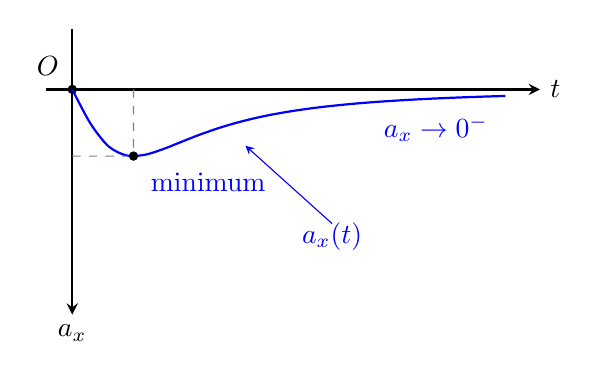
\begin{tikzpicture}[>=stealth, scale=1.1]
  % axes
  \draw[->, thick] (-0.3,0) -- (5.4,0) node[right] {$t$};
  \draw[->, thick] (0,0.7) -- (0,-2.6) node[below] {$a_x$};
  % origin marker
  \node[circle,fill,inner sep=1.2pt,label=above left:{$O$}] at (0,0) {};
  % curve
  \draw[domain=0.001:5.0,smooth,variable=\x,thick,blue]
    plot ({\x},{-2.0*\x/(1+\x*\x)^(1.5)});
  % extremum at t = 1/sqrt(2) ~= 0.707, a ~= -0.7698
  \node[circle,fill,inner sep=1.2pt] (M) at (0.707,-0.7698) {};
  \draw[dashed,gray] (0.707,0) -- (M);
  \draw[dashed,gray] (0,-0.7698) -- (M);
  \node[blue, below right=2pt of M] {minimum};
  % asymptote indicator
  \node[blue] at (4.2,-0.45) {$a_x\to 0^-$};
  % curve label, off the curve
  \node[blue] at (3.0,-1.7) {$a_x(t)$};
  \draw[blue,->,thin] (3.0,-1.55) -- (2.0,-0.65);
\end{tikzpicture}
\end{center}

\subsection*{(f) Fields and trajectory in the initial rest frame}

The initial rest frame $S^\star$ moves with $\bm V=(p_0/\gamma_0 m)\hat{\bm x}$, $\gamma_V=\gamma_0$. Apply the standard boost formulae to $\bm E=E_0\hat{\bm y}$, $\bm B=0$:
\[ E_y^\star = \gamma_0\,E_y = \gamma_0 E_0, \]
\[ B_z^\star = -\gamma_0\,\frac{V}{c^2}E_y = -\frac{\gamma_0 p_0 E_0}{m c^2}. \]
Hence
\begin{equation}
\boxed{\bm E^\star = \gamma_0 E_0\,\hat{\bm y},\qquad \bm B^\star = -\frac{\gamma_0 p_0 E_0}{m c^2}\hat{\bm z}.}
\end{equation}
At $t^\star=0$ the particle is at rest, so it accelerates along $+\hat{\bm y}$; once $v_y^\star>0$, the term $q\bm v\times\bm B^\star$ deflects it towards $-\hat{\bm x}$. Trajectory enters the second quadrant.

\medskip
\noindent\emph{Sketch of the spatial trajectory in $S^\star$:}
\begin{center}
\begin{tikzpicture}[>=stealth, scale=1.0]
  % axes
  \draw[->, thick] (-5.0,0) -- (1.2,0) node[right] {$x^\star$};
  \draw[->, thick] (0,-0.5) -- (0,3.8) node[above] {$y^\star$};
  % origin (start point) marker
  \node[circle,fill,inner sep=1.5pt,label=below right:{$O$}] at (0,0) {};
  % trajectory curve (cycloid-like, into second quadrant)
  \draw[thick,blue,domain=0:3.4,smooth,variable=\t]
    plot ({-0.6*(\t-0.4*sin(\t r))},{1.0*(1-cos(\t r))});
  % end-point marker
  \node[circle,fill,inner sep=1.2pt] (E) at ({-0.6*(3.4-0.4*sin(3.4 r))},{1.0*(1-cos(3.4 r))}) {};
  % curve label outside
  \node[blue] at (-3.6,3.2) {trajectory};
  \draw[blue,->,thin] (-3.4,3.05) -- (E);
  % initial tangent direction (along +y)
  \draw[->,red,thick] (0,0) -- (0,0.7) node[right,red] {$\bm v^\star(0^+)$};
\end{tikzpicture}
\end{center}

Asymptotically in $S$, $v_x\to 0$, $v_y\to c$. Boosting back,
\[ v_x^\star \to -V, \]
\[ v_y^\star \to c/\gamma_0. \]
Both finite, so the asymptote is a straight line of slope $-c/(\gamma_0 V) = -mc/p_0$; never vertical.

%==================================================================
\section*{Question 2 --- Doppler effect and resonant absorption with crossed source/detector motion}

\textbf{Problem statement.} Derive the relativistic Doppler formula. Then: source on $\bar y$-axis at speed $u$ through $\bar y_0$; detector on $\bar x$-axis at speed $v$. Work in the detector rest frame $S$: find the source's worldline, $v_{\rm rel}$, the emission/reception geometry, the frequency when the source crosses $S$'s $x$-axis, and the $u$ giving resonant absorption.

\subsection*{(a) The Doppler formula}

For the 4-frequency $K^\mu=(\omega/c)(1,\hat{\bm n})$ and source 4-velocity $U_{\rm src}$:
\[ \omega_0 = -\frac{K\cdot U_{\rm src}}{c} = \gamma_\beta\,\omega\,(1-\beta\cos\theta). \]
Solve for $\omega$:
\begin{equation}
\boxed{\omega = \frac{\omega_0\sqrt{1-\beta^2}}{1-\beta\cos\theta}.}
\label{eq:Q2a-2}
\end{equation}

\subsection*{(b) Trajectory of the source in the detector frame $S$}

Boost along $\bar{\bm x}$ at speed $v$, $\gamma=(1-v^2/c^2)^{-1/2}$. Source worldline in $\bar S$: $(\bar t,0,\bar y_0+u\bar t,0)$. Apply the inverse Lorentz transformation:
\[ t = \gamma\bar t, \]
\[ x = -v\,\gamma\,\bar t = -v\,t, \]
\[ y = \bar y_0 + u\bar t = \bar y_0 + u\,t/\gamma. \]
Hence
\begin{equation}
\boxed{\bm r_{\rm src}(t) = \bigl(-v t,\;\bar y_0 + u t/\gamma,\;0\bigr).}
\label{eq:Q2b-2}
\end{equation}

\subsection*{(c) Velocity of the source in $S$ and relative speed}

Differentiate \eqref{eq:Q2b-2}:
\[ \bm v_{\rm src}^{(S)} = \left(-v,\;u/\gamma,\;0\right). \]
The detector is at rest in $S$, so the relative speed is
\[ v_{\rm rel}^2 = v^2 + (u/\gamma)^2. \]
Substitute $1/\gamma^2 = 1-v^2/c^2$:
\[ v_{\rm rel}^2 = v^2 + u^2\,(1-v^2/c^2). \]
Take the square root:
\begin{equation}
\boxed{v_{\rm rel} = \sqrt{v^2 + u^2(1-v^2/c^2)}.}
\label{eq:Q2c-2}
\end{equation}
Limits: $v,u\ll c\Rightarrow\sqrt{v^2+u^2}$; $u\to c\Rightarrow v_{\rm rel}\to c$.

\subsection*{(d) Emission/reception geometry}

A photon emitted at $\bm r_{\rm src}(t)$ reaches the origin at $t_r$ with $|\bm r_{\rm src}(t)|=c(t_r-t)$. Square components:
\begin{equation}
\boxed{c(t_r-t) = \sqrt{v^2 t^2 + (\bar y_0 + ut/\gamma)^2}.}
\label{eq:Q2d-2}
\end{equation}
The angle $\theta$ between $\bm V_{\rm src}=(-v,u/\gamma,0)$ and the source-to-detector direction $-\bm r_{\rm src}(t)$ is obtained from
\[ v_{\rm rel}\,c(t_r-t)\cos\theta = \bm V_{\rm src}\cdot\bigl(-\bm r_{\rm src}(t)\bigr). \]
Expand the dot product:
\[ \bm V_{\rm src}\cdot\bigl(-\bm r_{\rm src}\bigr) = (-v)(vt) + (u/\gamma)\bigl(-\bar y_0 - ut/\gamma\bigr). \]
Collect:
\begin{equation}
\boxed{v_{\rm rel}\,c(t_r-t)\cos\theta = -v^2 t - \frac{u\bar y_0}{\gamma} - \frac{u^2 t}{\gamma^2}.}
\end{equation}

\medskip
\noindent\emph{Geometry in the detector frame $S$:}
\begin{center}
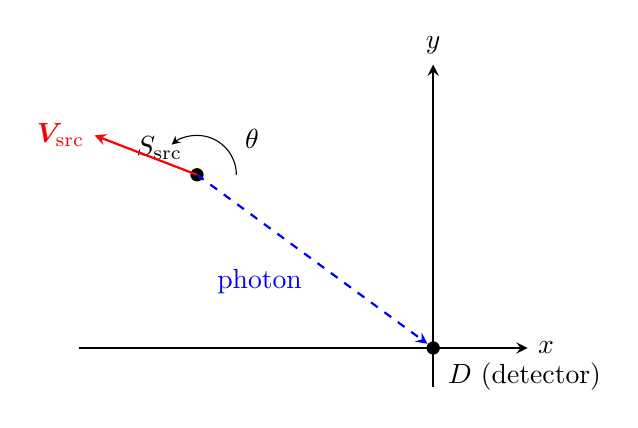
\begin{tikzpicture}[>=stealth, scale=1.0]
  % axes
  \draw[->, thick] (-4.5,0) -- (1.2,0) node[right] {$x$};
  \draw[->, thick] (0,-0.5) -- (0,3.6) node[above] {$y$};
  % detector at origin
  \node[circle,fill,inner sep=1.7pt,label=below right:{$D$ (detector)}] (D) at (0,0) {};
  % source position at emission
  \coordinate (Sp) at (-3.0,2.2);
  \node[circle,fill,inner sep=1.7pt,label=above left:{$S_{\rm src}$}] at (Sp) {};
  % source velocity
  \draw[->,red,thick] (Sp) -- ++(-1.3,0.5) node[left,red] {$\bm V_{\rm src}$};
  % photon path from source to detector
  \draw[->,blue,thick,dashed] (Sp) -- (D) node[midway,below left] {photon};
  % angle theta
  \draw[->,thin] (Sp) ++(0.5,0) arc[start angle=0,end angle=130,radius=0.5];
  \node at ($(Sp)+(0.7,0.45)$) {$\theta$};
\end{tikzpicture}
\end{center}

\subsection*{(e) Frequency observed when the source crosses the $x$-axis}

Set $y(t)=0$ in \eqref{eq:Q2b-2} to find the emission time:
\[ t_\star = -\gamma\bar y_0/u. \]
At this moment the source lies on the $x$-axis, so the photon to the detector at the origin propagates along $-\hat{\bm x}$. Project $\bm V_{\rm src}$ onto the source-to-detector direction $-\hat{\bm x}$:
\[ \bm V_{\rm src}\cdot(-\hat{\bm x}) = v. \]
Hence
\[ \cos\theta = \frac{\bm V_{\rm src}\cdot(-\hat{\bm x})}{v_{\rm rel}} = \frac{v}{v_{\rm rel}}. \]
Substitute into \eqref{eq:Q2a-2} with $\beta=v_{\rm rel}/c$:
\[ \omega = \frac{\omega_0\sqrt{1-v_{\rm rel}^2/c^2}}{1-v_{\rm rel}\cos\theta/c} = \frac{\omega_0\sqrt{1-v_{\rm rel}^2/c^2}}{1-v/c}. \]
Use $1-v_{\rm rel}^2/c^2 = (1-v^2/c^2)(1-u^2/c^2)$:
\[ \omega = \omega_0\,\frac{\sqrt{(1-v^2/c^2)(1-u^2/c^2)}}{1-v/c}. \]
Factor $1-v^2/c^2=(1-v/c)(1+v/c)$:
\[ \omega = \omega_0\,\sqrt{\frac{(1-v/c)(1+v/c)(1-u^2/c^2)}{(1-v/c)^2}}. \]
Cancel one $(1-v/c)$:
\begin{equation}
\boxed{\omega = \omega_0\sqrt{\frac{(1+v/c)(1-u^2/c^2)}{1-v/c}}.}
\label{eq:Q2e-4}
\end{equation}

\subsection*{(f) Resonant absorption}

Excited mass $M=m+\hbar\omega_0/c^2$. Conservation of 4-momentum on a stationary atom absorbing a photon of energy $\hbar\omega$ along $-\hat{\bm x}$ gives, after squaring,
\[ (mc+\hbar\omega/c)^2 - (\hbar\omega/c)^2 = M^2 c^2. \]
Expand the left-hand side:
\[ m^2 c^2 + 2m\hbar\omega + (\hbar\omega/c)^2 - (\hbar\omega/c)^2 = M^2 c^2. \]
Cancel the $(\hbar\omega/c)^2$ terms and substitute $M$:
\[ m^2 c^2 + 2m\hbar\omega = m^2 c^2 + 2m\,\frac{\hbar\omega_0}{c^2}c^2 + \left(\frac{\hbar\omega_0}{c^2}\right)^2 c^2. \]
Solve for $\omega$:
\[ \omega = \omega_0 + \frac{(\hbar\omega_0)^2}{2mc^2\,\hbar} = \omega_0\left(1+\frac{\hbar\omega_0}{2mc^2}\right). \]
Hence the recoil-shifted resonance condition:
\begin{equation}
\omega_{\rm res} = \omega_0\left(1+\frac{\hbar\omega_0}{2mc^2}\right).
\label{eq:Q2f-4}
\end{equation}
Equate \eqref{eq:Q2e-4} with \eqref{eq:Q2f-4}:
\[ \sqrt{\frac{(1+v/c)(1-u^2/c^2)}{1-v/c}} = 1+\frac{\hbar\omega_0}{2mc^2}. \]
Square both sides:
\[ \frac{(1+v/c)(1-u^2/c^2)}{1-v/c} = \left(1+\frac{\hbar\omega_0}{2mc^2}\right)^2. \]
Solve for $1-u^2/c^2$:
\[ 1-u^2/c^2 = \frac{1-v/c}{1+v/c}\left(1+\frac{\hbar\omega_0}{2mc^2}\right)^2. \]
Hence
\begin{equation}
\boxed{u = c\sqrt{1 - \frac{1-v/c}{1+v/c}\left(1+\frac{\hbar\omega_0}{2mc^2}\right)^2}.}
\end{equation}

%==================================================================
\section*{Question 3 --- 4-vectors, EM tensor, and stress-energy}

\textbf{Problem statement.} Identify which four-tuples are 4-vectors. Show that a 4-force preserves rest mass iff $F\cdot U=0$, and deduce antisymmetry of $\mathbb{G}$. With $\bm E\parallel\bm B$, $|\bm E|=E_0$, $|\bm B|=B_0=E_0/c$ in $S$, study the EM invariants and the stress-energy tensor in $S$ and a boosted frame $S'$.

\subsection*{(a) Which are 4-vectors?}

Multiplication by a Lorentz scalar preserves 4-vector character; multiplication by frame-dependent quantities does not.
\begin{itemize}
\item \textbf{1.} $X^\mu$ -- yes.
\item \textbf{2.} $(c,\bm v)$ -- no, missing $\gamma$.
\item \textbf{3.} $P^\mu=(E/c,\bm p)$ -- yes.
\item \textbf{4.} $m X^\mu$ -- yes ($m$ invariant).
\item \textbf{5.} $m(c,\bm v)$ -- no, missing $\gamma$.
\item \textbf{6.} $E(c,\bm v)$ -- no, $E$ frame-dependent.
\end{itemize}
\begin{equation}
\boxed{\text{4-vectors: 1, 3, 4. Not 4-vectors: 2, 5, 6.}}
\end{equation}

\subsection*{(b) Rest-mass preservation}

From $U\cdot U=-c^2$, differentiate:
\[ 2\,A\cdot U = 0,\qquad A\cdot U = 0. \]
With $F=\dot m\,U+m A$, dot with $U$:
\[ F\cdot U = \dot m\,(U\cdot U) + m\,(A\cdot U) = -\dot m\,c^2. \]
Hence $F\cdot U=0\Leftrightarrow\dot m=0$.

For $F=q\,\mathbb{G}\cdot U$, write
\[ F\cdot U = q\,U_a\,U_c\,\mathbb{G}^{ac}. \]
Symmetrise $U_aU_c$:
\[ F\cdot U = q\,U_a\,U_c\,\mathbb{G}^{(ac)}. \]
This vanishes for all $U$ iff
\begin{equation}
\boxed{\mathbb{G}^{ab} = -\mathbb{G}^{ba}.}
\end{equation}
This is why the Faraday tensor is antisymmetric.

\subsection*{(c) Invariants of the EM field with parallel $\bm E,\bm B$}

\begin{align}
I_1 &= \bm B^2 - \bm E^2/c^2, & I_2 &= -\bm E\cdot\bm B/c.
\end{align}
With $\bm E\parallel\bm B$, $|\bm E|=E_0$, $|\bm B|=E_0/c$, evaluate:
\[ I_1 = (E_0/c)^2 - E_0^2/c^2 = 0, \]
\[ I_2 = -E_0\,(E_0/c)/c = -E_0^2/c. \]
In any other frame $S^\dagger$, invariance gives $|\bm E^\dagger|^2/c^2 - |\bm B^\dagger|^2 = 0$, so
\[ |\bm E^\dagger| = c|\bm B^\dagger|, \]
and
\[ \bm E^\dagger\cdot\bm B^\dagger = E_0^2/c. \]
By Cauchy--Schwarz,
\[ E_0^2/c \leq |\bm E^\dagger||\bm B^\dagger| = c|\bm B^\dagger|^2. \]
Hence
\[ \boxed{|\bm B^\dagger|\geq B_0,\ |\bm E^\dagger|\geq E_0.} \]
For $|\bm B'|=\sqrt 2 B_0$, $|\bm E'|=\sqrt 2 E_0$:
\[ \cos\phi = \frac{\bm E'\cdot\bm B'}{|\bm E'||\bm B'|} = \frac{E_0^2/c}{\sqrt 2 E_0\cdot\sqrt 2 E_0/c} = \frac{1}{2}. \]
Hence
\begin{equation}
\boxed{\phi=\pi/3.}
\end{equation}

\medskip
\noindent\emph{Sketch of $\bm E'$ and $\bm B'$ in $S'$:}
\begin{center}
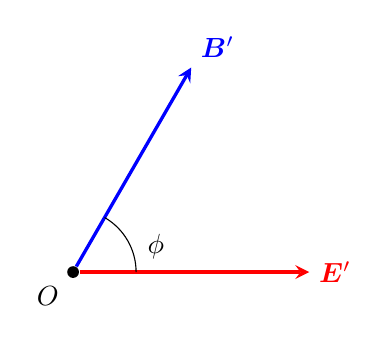
\begin{tikzpicture}[>=stealth, scale=1.0]
  % origin
  \node[circle,fill,inner sep=1.5pt,label=below left:{$O$}] (O) at (0,0) {};
  % E' along x
  \draw[->,very thick,red] (O) -- (3.0,0);
  \node[red,right] at (3.0,0) {$\bm E'$};
  % B' at 60 degrees
  \draw[->,very thick,blue] (O) -- ({3.0*cos(60)},{3.0*sin(60)});
  \node[blue,above right] at ({3.0*cos(60)},{3.0*sin(60)}) {$\bm B'$};
  % angle arc
  \draw[thin] (0.8,0) arc[start angle=0,end angle=60,radius=0.8];
  \node at (1.05,0.32) {$\phi$};
\end{tikzpicture}
\end{center}

\subsection*{(d) Stress-energy tensor in $S$}

$\bm E=E_0\hat{\bm y}$, $\bm B=(E_0/c)\hat{\bm y}$. Energy density:
\[ u = \tfrac12\epsilon_0 E_0^2 + \tfrac{1}{2\mu_0}(E_0/c)^2 = \tfrac12\epsilon_0 E_0^2 + \tfrac12\epsilon_0 E_0^2 = \epsilon_0 E_0^2. \]
Poynting vector:
\[ \bm S = \frac{1}{\mu_0}\bm E\times\bm B = 0 \quad(\text{parallel fields}). \]
Maxwell stress is diagonal: tension $-\epsilon_0 E_0^2$ along $\hat{\bm y}$, pressure $+\epsilon_0 E_0^2$ in $\hat{\bm x},\hat{\bm z}$. Hence
\begin{equation}
\mathbb{T} = \epsilon_0 E_0^2\begin{pmatrix} 1 & 0 & 0 & 0 \\ 0 & 1 & 0 & 0 \\ 0 & 0 & -1 & 0 \\ 0 & 0 & 0 & 1\end{pmatrix},
\end{equation}
\begin{equation}
\boxed{\mathbb{T}^{00}=\epsilon_0 E_0^2,\quad \mathbb{T}^{0i}=0,\quad \mathbb{T}^{xx}=\mathbb{T}^{zz}=+\epsilon_0 E_0^2,\quad \mathbb{T}^{yy}=-\epsilon_0 E_0^2.}
\end{equation}
Symmetry $\mathbb{T}^{0i}=\mathbb{T}^{i0}$: momentum density $=$ energy flux/$c^2$.

\subsection*{(e) Stress-energy in $S'$}

Boost along $\hat{\bm x}$ at $\beta=v/c$. Apply $\mathbb{T}'^{\mu\nu}=\Lambda^\mu{}_\alpha\Lambda^\nu{}_\beta\mathbb{T}^{\alpha\beta}$ to the $(t,x)$ block. Compute each entry:
\[ \mathbb{T}'^{00} = \gamma^2(\mathbb{T}^{00}+\beta^2\mathbb{T}^{xx}) = \epsilon_0 E_0^2\,\gamma^2(1+\beta^2), \]
\[ \mathbb{T}'^{0x} = -\gamma^2\beta(\mathbb{T}^{00}+\mathbb{T}^{xx}) = -2\epsilon_0 E_0^2\,\gamma^2\beta, \]
\[ \mathbb{T}'^{xx} = \gamma^2(\beta^2\mathbb{T}^{00}+\mathbb{T}^{xx}) = \epsilon_0 E_0^2\,\gamma^2(1+\beta^2). \]
Collect into the block form:
\begin{equation}
\begin{pmatrix} \mathbb{T}^{00\prime} & \mathbb{T}^{0x\prime}\\ \mathbb{T}^{0x\prime} & \mathbb{T}^{xx\prime}\end{pmatrix}
= \epsilon_0 E_0^2\,\gamma^2\begin{pmatrix}1+\beta^2 & -2\beta\\ -2\beta & 1+\beta^2\end{pmatrix},
\end{equation}
others unchanged. Hence
\begin{equation}
\boxed{\mathbb{T}'=\epsilon_0 E_0^2\begin{pmatrix}\gamma^2(1+\beta^2) & -2\gamma^2\beta & 0 & 0\\ -2\gamma^2\beta & \gamma^2(1+\beta^2) & 0 & 0\\ 0 & 0 & -1 & 0 \\ 0 & 0 & 0 & 1\end{pmatrix}.}
\end{equation}

\subsection*{(f) Energy flux at low velocity}

To first order in $v/c$, $\gamma\approx 1$. Read off:
\[ cT^{0x\prime} \approx -2v\,\epsilon_0 E_0^2, \]
\[ T^{00\prime} \approx \epsilon_0 E_0^2. \]
Pure convection $\rho v$ with $\rho = T^{00}/c^2\cdot c^2 = \epsilon_0 E_0^2$ alone would contribute
\[ \text{convective flux} = \rho v = \epsilon_0 E_0^2\,v\quad(\text{magnitude }\epsilon_0 E_0^2 v), \]
i.e.\ half the actual flux. The missing piece is the Maxwell stress doing work on moving surfaces: $\sigma_{xx}=-\epsilon_0 E_0^2$, contributing $-\sigma_{xx}v=\epsilon_0 E_0^2\,v$.
\begin{equation}
\boxed{\text{flux} = \underbrace{\rho v}_{-\epsilon_0 E_0^2 v} + \underbrace{(-\sigma_{xx})v}_{-\epsilon_0 E_0^2 v} = -2\epsilon_0 E_0^2 v.}
\end{equation}

%==================================================================
\section*{Question 4 --- Mandelstam variables, scattering kinematics, and free-particle action}

\textbf{Problem statement.} Elastic $\mathsf P+\mathsf Q\to\mathsf P'+\mathsf Q'$ with rest masses $m_1,m_2$. Develop Mandelstam variables, prove ZMF energy conservation, find $t,s,\cos\theta$. With $c=1$, treat the relativistic free particle: maximal-proper-time worldline, Lagrangian, Hamiltonian.

\subsection*{(a) Lorentz-invariant scalar products}

Square the conservation law $\mathsf P+\mathsf Q=\mathsf P'+\mathsf Q'$:
\[ \mathsf P^2 + 2\mathsf P\cdot\mathsf Q + \mathsf Q^2 = \mathsf P'^2 + 2\mathsf P'\cdot\mathsf Q' + \mathsf Q'^2. \]
Use $\mathsf P^2=\mathsf P'^2=-m_1^2 c^2$, $\mathsf Q^2=\mathsf Q'^2=-m_2^2 c^2$:
\[ 2\mathsf P\cdot\mathsf Q = 2\mathsf P'\cdot\mathsf Q'. \]
Hence
\begin{equation}
\boxed{\mathsf P\cdot\mathsf Q = \mathsf P'\cdot\mathsf Q'.}
\end{equation}
Square the rearrangement $\mathsf P-\mathsf Q'=\mathsf P'-\mathsf Q$:
\[ \mathsf P^2 - 2\mathsf P\cdot\mathsf Q' + \mathsf Q'^2 = \mathsf P'^2 - 2\mathsf P'\cdot\mathsf Q + \mathsf Q^2. \]
Cancel mass-shell terms:
\begin{equation}
\boxed{\mathsf P\cdot\mathsf Q' = \mathsf P'\cdot\mathsf Q.}
\end{equation}

\subsection*{(b) The sum $s+t+u$}

With $c=1$, expand each Mandelstam square:
\[ s = -(\mathsf P+\mathsf Q)^2 = m_1^2 + m_2^2 - 2\mathsf P\cdot\mathsf Q, \]
\[ t = -(\mathsf P-\mathsf P')^2 = 2 m_1^2 - 2\mathsf P\cdot\mathsf P', \]
\[ u = -(\mathsf P-\mathsf Q')^2 = m_1^2 + m_2^2 - 2\mathsf P\cdot\mathsf Q'\cdot(-1)\cdot\ldots \]
(using metric $(-+++)$ and rest masses), or equivalently
\[ u = m_1^2+m_2^2 -2\mathsf P\cdot\mathsf Q'. \]
Add the three:
\[ s+t+u = 4m_1^2 + 2m_2^2 - 2\mathsf P\cdot(\mathsf Q+\mathsf P'+\mathsf Q'). \]
Use 4-momentum conservation $\mathsf P'+\mathsf Q'=\mathsf P+\mathsf Q$:
\[ s+t+u = 4m_1^2 + 2m_2^2 - 2\mathsf P\cdot(2\mathsf P+2\mathsf Q-\mathsf P) = 2m_1^2 + 2m_2^2. \]
Hence
\begin{equation}
\boxed{s+t+u = 2m_1^2 + 2m_2^2.}
\end{equation}

\subsection*{(c) Energy conservation in the zero-momentum frame}

In the ZMF $\bm q=-\bm p$ and $\bm q'=-\bm p'$, with $E_i=\sqrt{m_i^2+|\bm p|^2}$. Compute
\[ E_1^2 - E_2^2 = m_1^2 - m_2^2, \]
\[ E_1'^2 - E_2'^2 = m_1^2 - m_2^2. \]
Subtract:
\[ E_1^2 - E_2^2 = E_1'^2 - E_2'^2. \]
Factor as $(E_1-E_2)(E_1+E_2)=(E_1'-E_2')(E_1'+E_2')$ and use total-energy conservation $E_1+E_2=E_1'+E_2'$:
\[ E_1 - E_2 = E_1' - E_2'. \]
Combine the sum and difference:
\begin{equation}
\boxed{E_1=E_1',\qquad E_2=E_2',}
\end{equation}
and consequently $|\bm p|=|\bm p'|$.

\subsection*{(d) $t$ and $\cos\theta$; $s$ in terms of energies}

In the ZMF, $\mathsf P-\mathsf P'=\mathsf Q'-\mathsf Q=(0,\bm q'-\bm q)$:
\begin{equation}
t = (\bm q'-\bm q)^2 = 2p^2(1-\cos\theta).
\label{eq:Q4d-1}
\end{equation}
Also, $\bm p+\bm q=0$ in the ZMF, so
\[ s = (E_1+E_2)^2. \]
Expand:
\[ s = E_1^2 + 2E_1 E_2 + E_2^2 = m_1^2 + m_2^2 + 2(E_1 E_2 + p^2). \]
From $E_1+E_2=\sqrt s$ and $E_1-E_2=(m_1^2-m_2^2)/\sqrt s$, multiply:
\[ E_1^2 - E_2^2 = m_1^2 - m_2^2, \]
and individually
\[ E_1 = \frac{s+m_1^2-m_2^2}{2\sqrt s},\qquad E_2 = \frac{s-m_1^2+m_2^2}{2\sqrt s}. \]
Multiply:
\[ E_1 E_2 = \frac{s^2 - (m_1^2-m_2^2)^2}{4s}. \]
Solve for $p^2$ from $s = m_1^2+m_2^2+2E_1E_2+2p^2$:
\[ p^2 = \frac{[s-(m_1+m_2)^2][s-(m_1-m_2)^2]}{4s}. \]
Substitute into \eqref{eq:Q4d-1}:
\[ t = 2p^2(1-\cos\theta), \]
\[ 1-\cos\theta = \frac{t}{2p^2} = \frac{2 s\, t}{[s-(m_1+m_2)^2][s-(m_1-m_2)^2]}. \]
Hence
\begin{equation}
\boxed{\cos\theta = 1 - \frac{2 s\, t}{[s-(m_1+m_2)^2][s-(m_1-m_2)^2]}.}
\end{equation}

\medskip
\noindent\emph{ZMF scattering geometry:}
\begin{center}
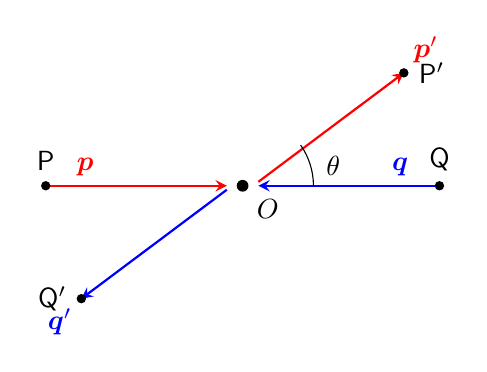
\begin{tikzpicture}[>=stealth, scale=1.0]
  % collision point
  \node[circle,fill,inner sep=1.5pt,label=below right:{$O$}] (O) at (0,0) {};
  % incoming P along +x
  \draw[->,thick,red] (-2.5,0) -- (-0.2,0);
  \node[red,above] at (-2.0,0) {$\bm p$};
  \node[circle,fill,inner sep=1.2pt,label=above:{$\mathsf P$}] at (-2.5,0) {};
  % incoming Q along -x
  \draw[->,thick,blue] (2.5,0) -- (0.2,0);
  \node[blue,above] at (2.0,0) {$\bm q$};
  \node[circle,fill,inner sep=1.2pt,label=above:{$\mathsf Q$}] at (2.5,0) {};
  % outgoing P' at angle theta
  \draw[->,thick,red] (0.2,0.05) -- ({2.5*cos(35)},{2.5*sin(35)});
  \node[red,above right] at ({2.5*cos(35)},{2.5*sin(35)}) {$\bm p'$};
  \node[circle,fill,inner sep=1.2pt,label=right:{$\mathsf P'$}] at ({2.5*cos(35)},{2.5*sin(35)}) {};
  % outgoing Q'
  \draw[->,thick,blue] (-0.2,-0.05) -- ({-2.5*cos(35)},{-2.5*sin(35)});
  \node[blue,below left] at ({-2.5*cos(35)},{-2.5*sin(35)}) {$\bm q'$};
  \node[circle,fill,inner sep=1.2pt,label=left:{$\mathsf Q'$}] at ({-2.5*cos(35)},{-2.5*sin(35)}) {};
  % angle arc
  \draw[thin] (0.9,0) arc[start angle=0,end angle=35,radius=0.9];
  \node at (1.15,0.25) {$\theta$};
\end{tikzpicture}
\end{center}

\subsection*{(e) Application to $p\bar p\to\pi\bar\pi$ and Lorentz invariance of probabilities}

Masses change ($m_p\neq m_\pi$), so part (a) no longer gives $E_1=E_1'$. The Mandelstam variables are still Lorentz invariants with $s+t+u=2m_p^2+2m_\pi^2$, and an analogous formula holds for $\cos\theta(s,t,m_p,m_\pi)$; $|\bm p|$ differs for in/out pairs.

A probability of obtaining $\pi\bar\pi$ versus $p\bar p$ is the ratio of two Lorentz-scalar quantities ($|\mathcal M|^2$ integrated over invariant phase space, divided by an invariant flux), so it is itself frame-invariant. Equivalently, ``which final state occurred'' is a frame-independent fact.

\subsection*{(f) Worldline of maximum proper time}

\[ \tau_{AB} = \int_A^B\sqrt{-\de X\cdot\de X}/c. \]
By the inverse triangle inequality for timelike vectors, $\tau$ is maximised by the geodesic, i.e.\ the
\begin{equation}
\boxed{\text{straight (inertial) worldline through } A\text{ and }B.}
\end{equation}

\subsection*{(g) Lagrangian and Hamiltonian for the free relativistic particle}

Take (with $c=1$)
\begin{equation}
L = -m\sqrt{1-\bm v^2},
\end{equation}
so $S=-m\int\de\tau$ is stationary on the maximal-$\tau$ worldline. Compute the canonical momentum:
\[ \bm p = \pd{L}{\bm v} = \frac{m\,\bm v}{\sqrt{1-\bm v^2}} = \gamma m\bm v. \]
Legendre transform:
\[ H = \bm p\cdot\bm v - L = \frac{m\,\bm v^2}{\sqrt{1-\bm v^2}} + m\sqrt{1-\bm v^2}. \]
Combine over a common denominator:
\[ H = \frac{m\,\bm v^2 + m(1-\bm v^2)}{\sqrt{1-\bm v^2}} = \frac{m}{\sqrt{1-\bm v^2}} = \gamma m. \]
Invert $\bm p=\gamma m\bm v$ for $\bm v$:
\[ \bm v = \frac{\bm p}{\sqrt{\bm p^2 + m^2}}. \]
Hence
\begin{equation}
\boxed{H(\bm p,\bm r) = \sqrt{\bm p^2 + m^2}\quad(c=1),\quad\text{or}\quad H=\sqrt{\bm p^2 c^2 + m^2 c^4}.}
\end{equation}
Non-relativistic limit: $H\approx mc^2 + \bm p^2/(2m)$.

\end{document}
